%%%%%%%%%%%%%%%%%%%%%%%%%%%%%%%%%%%%%%%%%%%%%%%%%%%%%%%%%%%%
%%  NE 155/255
%%

\documentclass[xcolor=x11names,compress,handout]{beamer}

\mode<handout>
{
  \usepackage{pgf}
  \usepackage{pgfpages}
  \pgfpagesuselayout{2 on 1}[a4paper,border shrink=5mm]
  \pgfpageslogicalpageoptions{1}{border code=\pgfusepath{stroke}}
\pgfpageslogicalpageoptions{2}{border code=\pgfusepath{stroke}}
}

\definecolor{CoolBlack}{rgb}{0.0, 0.18, 0.39}
%% General document %%%%%%%%%%%%%%%%%%%%%%%%%%%%%%%%%%
\usepackage{graphicx}
\usepackage{tikz}
\usetikzlibrary{decorations.fractals}
\usepackage{hyperref}
%%%%%%%%%%%%%%%%%%%%%%%%%%%%%%%%%%%%%%%%%%%%%%%%%%%%%%

%% Beamer Layout %%%%%%%%%%%%%%%%%%%%%%%%%%%%%%%%%%
\useoutertheme[subsection=false,shadow]{miniframes}
\useinnertheme{default}
% \usefonttheme{serif}
% \usepackage{palatino}
\usepackage{tabu}
\usepackage{ulem}
% Links
\usepackage{hyperref}
\definecolor{links}{HTML}{003262}
\hypersetup{colorlinks,linkcolor=,urlcolor=links}

% addition of color
\usepackage{xcolor}
\definecolor{CoolBlack}{rgb}{0.0, 0.18, 0.39}
\definecolor{byellow}{rgb}{0.55037, 0.38821, 0.06142}
\definecolor{dgreen}{rgb}{0.,0.6,0.}
\definecolor{RawSienna}{cmyk}{0,0.72,1,0.45}
\definecolor{forestgreen(web)}{rgb}{0.13, 0.55, 0.13}
\definecolor{cardinal}{rgb}{0.77, 0.12, 0.23}

\setbeamerfont{title like}{shape=\scshape}
\setbeamerfont{frametitle}{shape=\scshape}

\setbeamercolor*{lower separation line head}{bg=CoolBlack}
\setbeamercolor*{normal text}{fg=black,bg=white}
\setbeamercolor*{alerted text}{fg=dgreen}
\setbeamercolor*{example text}{fg=black}
\setbeamercolor*{structure}{fg=black}

\setbeamercolor*{palette tertiary}{fg=black,bg=black!10}
\setbeamercolor*{palette quaternary}{fg=black,bg=black!10}

% Margins
\usepackage{changepage}

\mode<presentation>
{
  \definecolor{berkeleyblue}{HTML}{003262}
  \definecolor{berkeleygold}{HTML}{FDB515}
  \usetheme{Boadilla}      % or try Darmstadt, Madrid, Warsaw, Boadilla...
  %\usecolortheme{dove} % or try albatross, beaver, crane, ...
  \setbeamercolor{structure}{fg=berkeleyblue,bg=berkeleygold}
  \setbeamercolor{palette primary}{bg=berkeleyblue,fg=white} % changed this
  \setbeamercolor{palette secondary}{fg=berkeleyblue,bg=berkeleygold} % changed this
  \setbeamercolor{palette tertiary}{bg=berkeleyblue,fg=white} % changed this
  \usefonttheme{structurebold}  % or try serif, structurebold, ...
  \useinnertheme{circles}
  \setbeamertemplate{navigation symbols}{}
  \setbeamertemplate{caption}[numbered]
  \usebackgroundtemplate{}
}
%---

\renewcommand{\(}{\begin{columns}}
\renewcommand{\)}{\end{columns}}
\newcommand{\<}[1]{\begin{column}{#1}}
\renewcommand{\>}{\end{column}}

% adding slide numbers
\addtobeamertemplate{navigation symbols}{}{%
    \usebeamerfont{footline}%
    \usebeamercolor[fg]{footline}%
    \hspace{1em}%
    \insertframenumber/\inserttotalframenumber
}

% equation stuff
\newcommand{\Macro}{\ensuremath{\Sigma}}
\newcommand{\Sn}{\ensuremath{S_N} }
\newcommand{\vOmega}{\ensuremath{\hat{\Omega}}}
\usepackage{mathrsfs}
\usepackage[mathcal]{euscript}
\usepackage{amssymb}
\usepackage{amsthm}
\usepackage{epsfig}
\usepackage{amsmath}
%%%%%%%%%%%%%%%%%%%%%%%%%%%%%%%%%%%%%%%%%%%%%%%%%%
% title stuff for footer
\title{NE 155/255}
\author{Kelly L.\ Rowland}
\date{November 6, 2019}

\begin{document}

%%%%%%%%%%%%%%%%%%%%%%%%%%%%%%%%%%%%%%%%%%%%%%%%%%%%%%
%%%%%%%%%%%%%%%%%%%%%%%%%%%%%%%%%%%%%%%%%%%%%%%%%%%%%%
\begin{frame}
\title{NE 155/255\\Numerical Simulations in Radiation Transport}
\subtitle{Introduction to Monte Carlo}
\titlepage
\end{frame}


%%%%%%%%%%%%%%%%%%%%%%%%%%%%%%%%%%%%%%%%%%%%%%%%%%%%%%
%%%%%%%%%%%%%%%%%%%%%%%%%%%%%%%%%%%%%%%%%%%%%%%%%%%%%%
\begin{frame}{Mathematical Validity}

\begin{itemize}
\item Consider particles with a phase space
describing position, $\vec{r}$, and velocity, $\vec{v}$
\vspace*{0.5 em}
\item A neutral particle can be transmitted
from one position to another at a
constant velocity
\[T(\vec{r}\:' \rightarrow \vec{r}, \vec{v})\]

\item A particle can undergo a collision at a
single position that changes its velocity
\[C(\vec{r}, \vec{v}\:' \rightarrow \vec{v})\]
\item Integral TE:
\[\psi(\vec{r}, \vec{v}) = \int_{\vec{r}\:'} \biggl[ \int_{\vec{v}\:'} \psi(\vec{r}\:', \vec{v}\:') C(\vec{r}\:', \vec{v}\:' \rightarrow \vec{v})  d\vec{v}\:'\biggr] T(\vec{r}\:' \rightarrow \vec{r}, \vec{v}) d\vec{r}\:'\]
\end{itemize}
\end{frame}


%%%%%%%%%%%%%%%%%%%%%%%%%%%%%%%%%%%%%%%%%%%%%%%%%%%%%%
%%%%%%%%%%%%%%%%%%%%%%%%%%%%%%%%%%%%%%%%%%%%%%%%%%%%%%
\begin{frame}{Can Model Very Complex Things}

  	\begin{figure}
  	\begin{center}
  		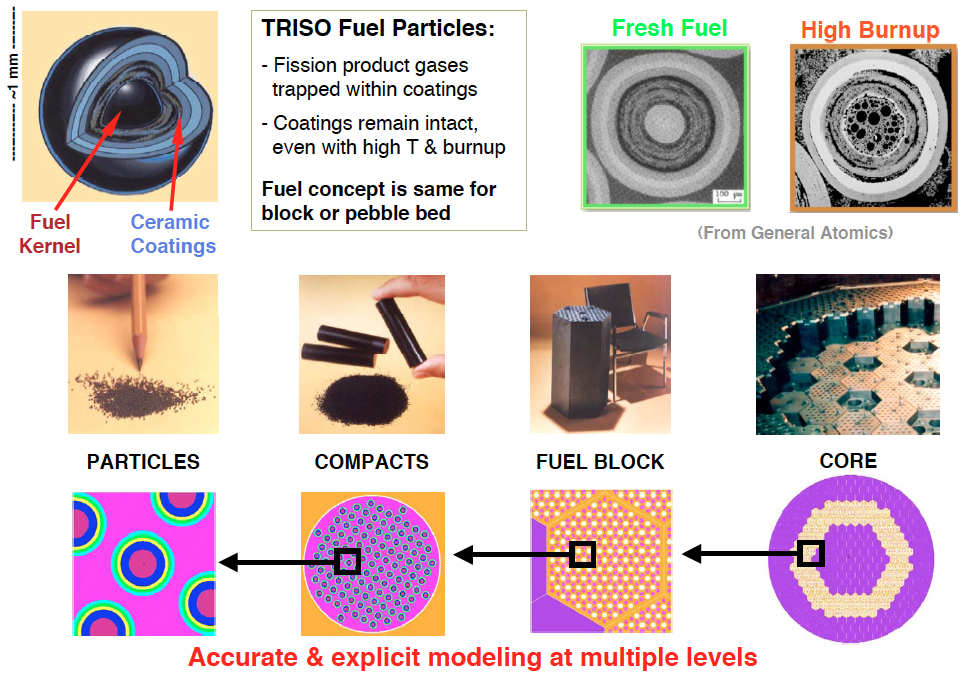
\includegraphics[height=3in,clip]{fig/pbmr}
	\end{center}
  	\end{figure}

\end{frame}

%%%%%%%%%%%%%%%%%%%%%%%%%%%%%%%%%%%%%%%%%%%%%%%%%%%%%%
%%%%%%%%%%%%%%%%%%%%%%%%%%%%%%%%%%%%%%%%%%%%%%%%%%%%%%
\begin{frame}{Major Components of MC Algorithm}

\begin{itemize}
  \item \textbf{PDFs}: the physical/mathematical system must be described by a set of pdfs.
  % That's next class
  
  \item \textbf{Random number generator}: a source of random \#s uniformly distributed on the unit interval.
  % We're going to skip this
  
  \item \textbf{Sampling rule}: prescription for sampling the pdf (given having random \#s)
  % That's also next class
  
  \item \textbf{Scoring}: the outcomes must be accumulated/\underline{tallied} for quantities of interest
  % we might cover it
  
  \item \textbf{Error estimation}: an estimate of the statistical error (\underline{variance}) of the solution
  % This class!
    
  \item \textbf{Variance Reduction}: methods for reducing the variance and computation time simultaneously
  % briefly this class, maybe more at the end
    
  \item \textbf{Parallelization}: efficient use of computers
  % probably not
\end{itemize}
\end{frame}



%%%%%%%%%%%%%%%%%%%%%%%%%%%%%%%%%%%%%%%%%%%%%%%%%%%%%%
%%%%%%%%%%%%%%%%%%%%%%%%%%%%%%%%%%%%%%%%%%%%%%%%%%%%%%
\begin{frame}{Basic Event-Based Algorithm}

\begin{figure}[h!]
\begin{center}
  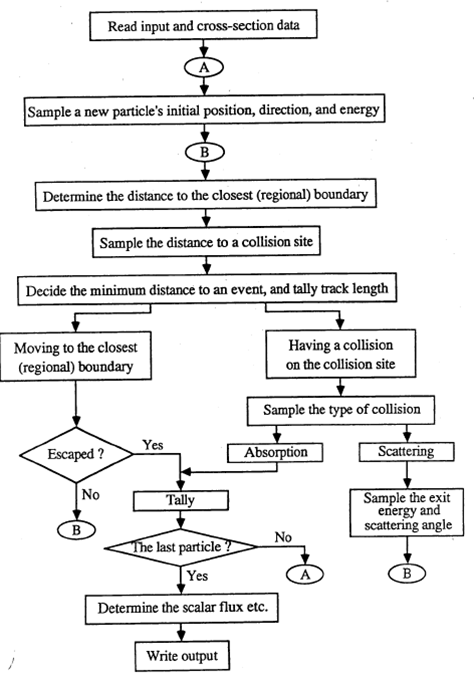
\includegraphics[height=3 in,clip]{fig/MC-algorithm}
\end{center}
  \label{fig:mc-algo}
\end{figure}

\end{frame}

%%%%%%%%%%%%%%%%%%%%%%%%%%%%%%%%%%%%%%%%%%%%%%%%%%%%%%
%%%%%%%%%%%%%%%%%%%%%%%%%%%%%%%%%%%%%%%%%%%%%%%%%%%%%%
\begin{frame}{Let's Get Started With...}

    \begin{enumerate}
    \item Physics as Probability
    \item Definitions: PDF \& CDF
    \item Motivation \& Goal of Random Sampling
    \item Basic Random Sampling Techniques
      \begin{itemize}
        \item Direct Discrete Sampling
        \item Direct Continuous Sampling
        \item Rejection Sampling
      \end{itemize}
    \end{enumerate}

\vspace*{1em}
Notes derived from Rachel Slaybaugh, Jasmina Vujic, and Paul Wilson.
\end{frame}



%%%%%%%%%%%%%%%%%%%%%%%%%%%%%%%%%%%%%%%%%%%%%%%%%%%%%%
%%%%%%%%%%%%%%%%%%%%%%%%%%%%%%%%%%%%%%%%%%%%%%%%%%%%%%
\begin{frame}{Learning Objectives}

    \begin{enumerate}
    \item Provide examples of probabilistic
representations of physics
    \item Distinguish between a PDF and CDF
    \item Distinguish between a \textit{discrete} PDF
(CDF) and \\ a \textit{continuous} PDF (CDF)
    \item Describe the goal of random sampling
    \item Identify and implement the best
random sampling technique for a given
distribution
    \end{enumerate}

\end{frame}


%%%%%%%%%%%%%%%%%%%%%%%%%%%%%%%%%%%%%%%%%%%%%%%%%%%%%%
%%%%%%%%%%%%%%%%%%%%%%%%%%%%%%%%%%%%%%%%%%%%%%%%%%%%%%
\begin{frame}{Physics as Probability}

Various physical phenomena can be
represented by probability distributions

\begin{itemize}
  \item Photon emission energy
    \begin{itemize}
    \item Each possible energy has a different probability
(intensity)
    \end{itemize} 
    
    \vspace*{0.5 em}
  \item Scattering cross-sections
    \begin{itemize}
    \item Each possible scattering angle has a different
probability as a function of the energy
    \end{itemize}
    
    \vspace*{0.5 em}
  \item Transmission through a medium
    \begin{itemize}
    \item Probability of reaching a particular position
depends on the cross-section
    \end{itemize}
\end{itemize}
\end{frame}


%%%%%%%%%%%%%%%%%%%%%%%%%%%%%%%%%%%%%%%%%%%%%%%%%%%%%%
%%%%%%%%%%%%%%%%%%%%%%%%%%%%%%%%%%%%%%%%%%%%%%%%%%%%%%
\begin{frame}{Probability Density Functions}

All variables, $x$, have a \underline{Probability Density Function (PDF)}, $p(x)$, with the following characteristics:

\begin{columns}[t]
  \begin{column}{0.5\textwidth}
    \begin{center}
    \textcolor{berkeleygold}{\underline{Continuous}} 
    \end{center}
    %
    \begin{align*}
    p\left\lbrace a \leq x \leq b \right\rbrace &= \int_a^b p(x)dx\\
    & \\
    p(x) & \geq 0 \\
    \int_{-\infty}^{\infty} p(x)dx &= 1
    \end{align*}
  \end{column}
  \begin{column}{0.5\textwidth}
    \begin{center}
    \textcolor{berkeleyblue}{\underline{Discrete}}  
    \end{center}
    %
    \begin{align*}
    p(x = x_k) &= p_k \equiv p(x_k)\\
    k &= 1, \dots, N \\
    & \\
    p_k & \geq 0 \\
    \sum_{k=1}^N p_k &= 1
    \end{align*}
  \end{column}
\end{columns}

\end{frame}


%%%%%%%%%%%%%%%%%%%%%%%%%%%%%%%%%%%%%%%%%%%%%%%%%%%%%%
%%%%%%%%%%%%%%%%%%%%%%%%%%%%%%%%%%%%%%%%%%%%%%%%%%%%%%
\begin{frame}{Cumulative Distribution Functions}

All PDFs, $p(x)$, have an associated \underline{Cumulative Distribution Function (CDF)}, $P(x)$, with the following properties:

\begin{columns}[t]
  \begin{column}{0.5\textwidth}
    \begin{center}
    \textcolor{berkeleygold}{\underline{Continuous}} 
    \end{center}
    %
    \begin{align*}
    P\left\lbrace x' \leq x \right\rbrace &= P(x) = \int_{-\infty}^x p(x')dx'\\
    & \\
    P(-\infty) &= 0 \:,\quad P(\infty) = 1 \\
    0 &\leq P(x) \leq 1 \\
    &\frac{dP(x)}{dx} \geq 0
    \end{align*}
  \end{column}
  \begin{column}{0.5\textwidth}
    \begin{center}
    \textcolor{berkeleyblue}{\underline{Discrete}}  
    \end{center}
    %
    \begin{align*}
    P\left\lbrace x' \leq x \right\rbrace &= P_k \equiv P(x_k) = \sum_{j=1}^k p_j\\
    k &= 1, \dots, N \\
    P_0 &= 0 \:,\quad P_N = 1 \\
    0 &\leq P_k \leq 1 \\
    P_k & \geq P_{k-1} \\
    \end{align*}
  \end{column}
\end{columns}

\end{frame}

\end{document}
